\documentclass[11pt]{article}
\usepackage{amsmath, amsfonts, amsthm, amssymb}  % Some math symbols
\usepackage{enumerate}
\usepackage{fullpage}
\usepackage{color}
\usepackage[x11names, rgb]{xcolor}
\usepackage{tikz}
\usepackage{graphicx}
\usepackage{listings}
\usepackage{fancyhdr}
\usepackage{pdflscape}
\usepackage{hyperref}

% \usepackage{fontspec}
% \setmainfont{Times New Roman}

\renewcommand*{\familydefault}{\sfdefault}

\setlength{\parindent}{0pt}
\setlength{\parskip}{6pt}
\pagestyle{empty}

\pagestyle{fancy}
\fancypagestyle{firststyle}
{
   \lhead{\myname \\ \myandrew \\ \today \\ \vspace*{-.5em}}
   \rhead{15-221 \\ Fall 2014 \\ Section A \\ \vspace*{-.5em}}
   \setlength{\headsep}{50pt}
}

\fancypagestyle{zerostyle}
{
   \renewcommand{\headrulewidth}{0pt}
}

\newcommand{\myname}{Justin Gallagher, Ted Li, Jacob Zimmerman, Howard Chen}
\newcommand{\myandrew}{Group 20}
\newcommand{\mytitle}{Project Proposal}
\title{ExplainShell for Chrome \\ \vspace*{.5em} \Large\mytitle}
\date{}
%%%%%%%%%%%%%%%%%%%%%%%%%%%%%%%%%%%%%%%%%%%%%%%%%%%%%%%%%%%

\begin{document}
\clearpage
\pagenumbering{gobble}
\thispagestyle{zerostyle}
4716 Ellsworth Avenue\\
Apartment 202\\
Pittsburgh, PA 15213\\

\today\\

Mr. Thomas M. Keating\\
Assistant Teaching Professor\\
School of Computer Science\\

Dear Mr. Keating:\\

Please find attached to this letter our team's proposal for ExplainShell for Chrome. The proposal will outline the details of this Google Chrome extension and demonstrate our plan for its execution, as well as testing and evaluation criteria.\\

The document contains an abstract, an introduction, a literature review, a plan, a discussion of the project's benefits, our approach, evaluation criteria, and the qualifications of our team members.\\

Please direct any questions or comments about the proposal to jrgallag@andrew.cmu.edu.\\

Sincerely,\\

~\\

Justin Gallagher
\vfill
enclosure: paper entitled ExplainShell for Chrome
\newpage

\pagenumbering{gobble} 
\author{~\\
\normalsize {\bf Submitted to}\\
\normalsize Thomas M. Keating\\
\normalsize Assistant Teaching Professor\\
\normalsize School of Computer Science\\
\normalsize Carnegie Mellon University\vspace*{2em}\\
\normalsize {\bf Prepared by}\\
\normalsize Justin Gallagher (author)\\
\normalsize Ted Li (author)\\
\normalsize Jacob Zimmerman\\
\normalsize Howard Chen\vspace*{2em}\\
\normalsize School of Computer Science\\
\normalsize Carnegie Mellon University\\
\normalsize \today}

\clearpage\maketitle
\thispagestyle{firststyle}

\begin{center}
\textbf{Abstract}
\end{center}

This paper is a proposal for ExplainShell for Chrome, a Google Chrome extension which helps users understand shell commands found online. Instead of blindly running commands found on the internet, the user can learn more thoroughly what they do. This prevents malicious commands from being run, and imparts the user with valuable knowledge. The proposal details our specific goals, approach, and schedule for completing the project.
\newpage
\lhead{\myname}
\rhead{\thepage}
\setlength{\headsep}{25pt}
\tableofcontents
\newpage
\pagenumbering{arabic} 
\setlength{\voffset}{-50pt}
\setlength{\headsep}{25pt}

\section{Introduction}
ExplainShell for Chrome will be a Google Chrome extension which aids users in learning and analyzing shell commands found online. When looking for help with Unix based systems, many users search the internet for answers, and use commands found on online forums and Q\&A centers without the proper understanding of their function. This can result in the user unknowingly running malicious or insecure commands. In addition, running commands this way prevents users from learning how to write such commands themselves. Documentation for shell commands exists in \texttt{man} pages and in resources such as explainshell.com, but this would require the user to retype the command or copy and paste to another webpage. This barrier is often too large for people who look up many commands.

ExplainShell for Chrome alleviates this problem by showing the user a popup window with a detailed explanation of commands found online. Utilizing information from explainshell.com, the extension will eliminate the need to copy and paste to another page. This project will provide a useful product and allow us to explore Chrome extension development as well as learn how to interact with other open source projects.

\section{Literature Review}

\subsection{explainshell.com and man pages}

\texttt{man} pages are the form of documentation used to store information about Unix software, including commands. These pages are very comprehensive, containing very detailed information about the command, including its effect, options and input types. However, it is often difficult to determine which part of the page relates to your command, and difficult to discover new commands the user was unaware of.

explainshell.com is a website which attempts to resolve this problem. Given a shell command, the website parses it into its component parts, and pulling up the appropriate section of the \texttt{man} page for each part. It displays this information in a simple, graphical format for easy understanding. However, the site requires users to navigate away from their page and copy-paste the command to analyze.

\subsection{bashoneliners.com}

bashoneliners.com is a website where users can submit one line shell commands the execute various functions. These commands are sorted by popularity, and accompanied by a detailed explanation of how they work written by the creator. However, this format means the site is naturally limited to what has been previously submitted. Descriptions must be written by humans, and so have a high quality but limited availability. It is also often difficult to find an already submitted command which does what the user is looking for.

\subsection{linuxcommand.org}

linuxcommand.org is a website that provides an in-depth tutorial for readers to learn how to write shell commands. The site aims to give users enough knowledge that they can write any commands needed themselves. However, there are still some specialized commands not covered by the lessons. In addition, it is difficult to quickly look through the site to find the explanation of a specific command.

\subsection{The Linux Documentation Project}

The website of The Linux Documentation Project, tldp.org, provides detailed free documentation for the GNU/Linux operating system and software. The project takes the form of a searchable wiki, which provides detailed information about specific commands and software. However, using the site requires users to parse commands themselves, and combine data from many different pages to form a picture of how a certain command would act.

\subsection{Chrome Extension Developers' Portal}

The Google Chrome Developers' site will be an invaluable resource to our project. The website offers a tutorial on building Chrome extensions and provide the documentation for Chrome. As none of us have written a Chrome extension before, we will need to use the site to get up to speed.

\section{Plan}

Our goal is to develop a Chrome extension that helps users learn the usage of shell commands found online and avoid malicious shell commands. After the user installs the extension from the Chrome extension store, it will scan any web page that the user visits for shell commands in the background, and allow users to simply hover / click on unfamiliar shell commands to view a detailed explanation of the shell commands in a pop-up window. This extension will not only help users learn and familiarize themselves with the usage of nearly 30,000 shell commands, but will also help users identify potentially destructive or malicious commands before executing them. 

We will also create a back-end server to store and provide interesting analytics about trending shell commands, trending referring sites and other statistics. If time allows, we will also attempt to develop a more advanced web page parsing technique to identify shell commands in a web page, possibly using machine learning.

For this project, we have set up a Git repository that allows us to coordinate and keep track of code changes easily. We have also set up a Google Drive to keep track of our progress. We will set up team meetings at the end of each phase by email or texting.

\section{Benefits}

This project will benefit both our team and end users. For users, the project will provide a convenient way to look up and learn the usage of unfamiliar shell commands found online. Considering that shell commands are often powerful and can sometimes be malicious, the project can also potentially automatically warn users about malicious shell commands before they execute the commands. 

We will learn to use and familiarize with a lot of technologies in the process as well, including Git, Chrome extension, Javascript and Python. Through the process, we will also contribute to the ExplainShell open source project.

\section{Approach}
\subsection{Methodology}

In this section, we will explain the various technologies that we will be using to complete the project. Through our project, we will develop a Chrome extension and a back-end server that provides analytics about trending shell commands. We will also contribute to the current code base of the open source ExplainShell project. 

For the Chrome extension, we will use Javascript and jQuery to scan and parse the webpage that user visits, to identify potential shell commands within a web page. We will then use AJAX to send requests to the ExplainShell API and receive documentations of identified commands. We will also use HTML + CSS to layout a pop-up window that displays the documentation. 

We will also create a back-end server with Node.js. The back-end server will store the history of shell commands that users look up using our extension, using a SQL database. The data will allow us to provide analytics and visualization about popular or trending searches.

\subsection{Project Schedule}
Specifically, our project will be separated into the following four phases. 

\par{\bf Phase 1}\\ 
We will first build a simple Chrome extension that allows user to look up the usage of shell command by selecting and highlighting any text in the browser window. Upon highlighting, a button will appear next to the highlighted text region. The user may click the button, which will instantly redirect the user to the corresponding usage documentation at the ExplainShell website in a new browser tab.

\par{\bf Phase 2}\\
We will refine our Chrome extension developed in Phase 1. Instead of asking the user to highlight the shell command that they want to look up, the Chrome extension will now automatically parse and search the web page to identify any shell commands. Upon identifying potential commands, the extension will turn the command into a clickable link, which will redirect the user to the usage documentation at the ExplainShell website.

\par{\bf Phase 3}\\
We will contribute to the code base of the ExplainShell project by adding a RESTful HTTP API, since this would also help us further improve our chrome extension. With the API, the Chrome extension may now display a pop-up window in the page, whenever the user hovers/clicks on the identified shell commands, whereas previously we always redirect the user to the documentation web page.

\par{\bf Phase 4}\\
We will develop a back-end server that provides analytics that allow users to view trending searches and referral sites. These analytics will provide insight in which shell commands people take most interest in or are confused about.

Please refer to Fig. \ref{fig:timetable} on page \pageref{fig:timetable} for a Gantt chart of our project schedule.

\section{Evaluation}

Our goal is to create a user-friendly Chrome extension and to eventually publish it onto the Chrome extension store. Interested users may download the ExplainShell Chrome extension. On one hand, we will ask our friends and classmates to help evaluate our extension, on its utility and ease of use. On the other hand, we will also request feedbacks from users who downloaded our extension from the Chrome extension store.

\section{Qualifications}

Overall, our team members have been previously been exposed to relevant technologies. Jacob had 1 year of full-stack web development and interned at Bloomberg L.P. working on software engineering. Justin has 2 years of HTML/CSS/Javascript experience and had a summer internship at Microsoft working on ASP.NET web applications using SQL databases. Ted has experience in iOS and web programming and interned at Bloomberg L.P. working on a project related to natural language processing. Howard has strong background in algorithmic thinking and taught Principles of Programming and Software Development this summer. 

There may be specific technologies that we are unfamiliar with, but they should be easy to pick up and would definitely be a good learning experience for us.

\begin{landscape}
\thispagestyle{empty}
\begin{figure}[htb]
\vspace*{6em}
\hspace*{-3em}
\centering
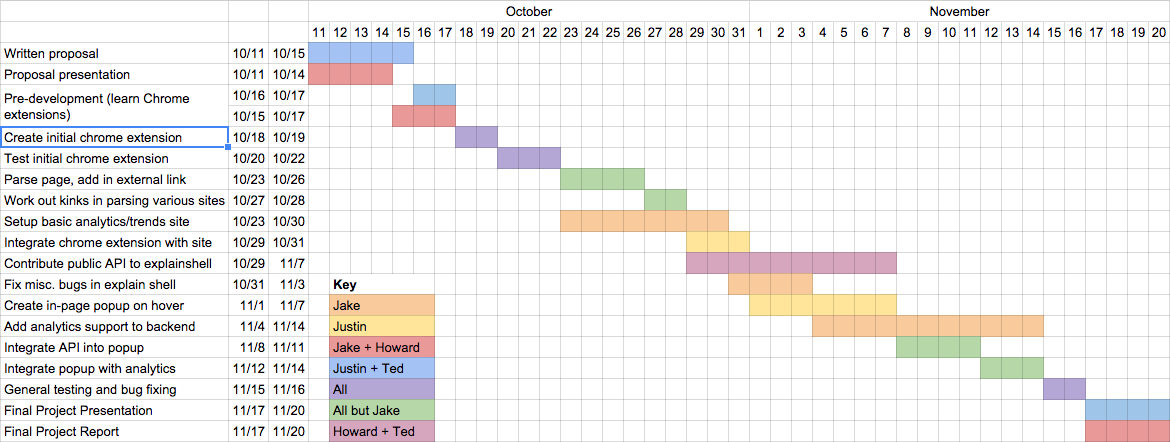
\includegraphics[width=1.5\textwidth]{gantt-chart.png}
\caption{Project time line\label{fig:timetable}}
\end{figure}
\end{landscape}

\begin{thebibliography}{9}

\bibitem{explainshell}
  ``ExplainShell project -- write down a command-line to see the help text that 
  matches each argument'',
  \url{http://explainshell.com/}

\bibitem{bashoneliners}
  ``Bash One-liners project'',
  \url{http://bashoneliners.com/}

\bibitem{linuxcommand}
  ``Linux commands -- beginner's tutorial to the command line environment'',
  \url{http://linuxcommand.org/}

\bibitem{tldp}
  ``TLDP -- widespread documentation on all things Linux'',
  \url{http://tldp.org/}

\bibitem{chromedev}
  ``Chrome Developers: Extensions Overview'',
  \url{https://developer.chrome.com/extensions/overview}

\end{thebibliography}

\end{document}
